\documentclass{standalone}
\usepackage{tikz}
\usetikzlibrary{shapes,arrows.meta}
\begin{document}
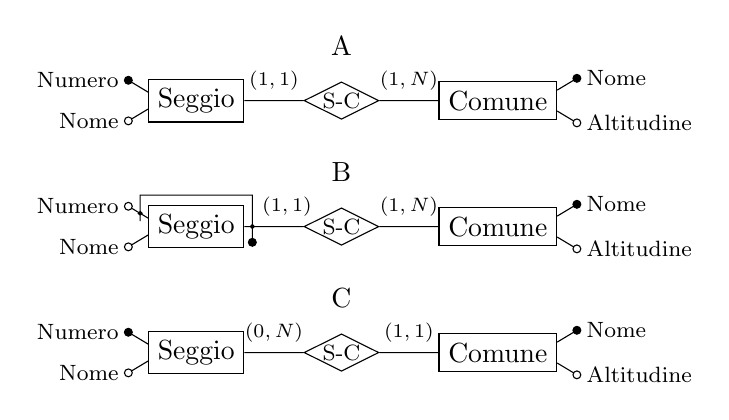
\begin{tikzpicture}
    \draw

    %%* Attributi:
    %%  node[draw, circle, inner sep=1pt, fill=black]{}node[right]{\footnotesize A}
    %%? Distanza orizzontale: E -(0.25,0.x)- A
    %%? Distanza verticale: E -(0,x * 0.22)- A

    %%* Cardinalità:
    %%  node[below right]{\scriptsize $(0,N)$}
    %%  node[above right]{\scriptsize $(0,N)$}
    %%  node[midway, above]{\scriptsize $(0,N)$}

    %%* Relazione:
    %%  node[draw, diamond, shape aspect=2, inner sep=3pt, anchor=90](r1){}
    %%  node[draw, diamond, shape aspect=2, inner sep=0.2pt, anchor=180](r2){R2}

    %%* Entità:
    %%  node[draw, rectangle, anchor=90](e1){}
    %%? Distanza verticale: E -(0.3)- R -(0.3) E
    %%? Distanza orizzontale: E -(0.75)- R -(0.75)- E

    %%* A:
    (0,0)node[draw, rectangle, anchor=180](seg){Seggio}
    (seg.190)--++(-0.25,-0.15)node[draw, circle, inner sep=1pt, fill=white]{}node[left]{\footnotesize Nome}
    (seg.170)--++(-0.25,0.15) node[draw, circle, inner sep=1pt, fill=black]{}node[left]{\footnotesize Numero}

    (seg.0)--++(0.75,0)node[draw, diamond, shape aspect=2, inner sep=0.4pt, anchor=180](r1){\footnotesize S-C}node[midway, above]{\scriptsize $(1,1)$}
    (r1.90)++(0,.2)node[above]{A}

    (r1.0)--++(0.75,0)node[draw, rectangle, anchor=180](com){Comune}node[midway, above]{\scriptsize $(1,N)$}
    (com.350)--++(0.25,-0.15)node[draw, circle, inner sep=1pt, fill=white]{}node[right]{\footnotesize Altitudine}
    (com.10)--++ (0.25,0.15) node[draw, circle, inner sep=1pt, fill=black]{}node[right]{\footnotesize Nome}


    %%* B:
    (0,-1.6)node[draw, rectangle, anchor=180](seg){Seggio}
    (seg.190)--++(-0.25,-0.15)node[draw, circle, inner sep=1pt, fill=white]{}node[left]{\footnotesize Nome}
    (seg.170)--++(-0.1,0.06)node[draw, circle, inner sep=0.5pt, fill=black](b){}--++(-0.15,0.09)node[draw, circle, inner sep=1pt, fill=white]{}node[left]{\footnotesize Numero}

    (seg.0)--++(0.1,0)node[above right]{\scriptsize $(1,1)$}
    node[draw, circle, inner sep=0.5pt, fill=black](a){}--++(0.65,0)node[draw, diamond, shape aspect=2, inner sep=0.4pt, anchor=180](r1){\footnotesize S-C}
    (r1.90)++(0,.2)node[above]{B}

    (r1.0)--++(0.75,0)node[draw, rectangle, anchor=180](com){Comune}node[midway, above]{\scriptsize $(1,N)$}
    (com.350)--++(0.25,-0.15)node[draw, circle, inner sep=1pt, fill=white]{}node[right]{\footnotesize Altitudine}
    (com.10) --++(0.25,0.15) node[draw, circle, inner sep=1pt, fill=black]{}node[right]{\footnotesize Nome}

    (a)++(0,-0.2)node[draw, circle, inner sep=1pt, fill=black]{}--++(0,0.6)-|(b)--++(0,-0.1)
    %%* C:
    (0,-3.2)node[draw, rectangle, anchor=180](seg){Seggio}
    (seg.190)--++(-0.25,-0.15)node[draw, circle, inner sep=1pt, fill=white]{}node[left]{\footnotesize Nome}
    (seg.170)--++(-0.25,0.15) node[draw, circle, inner sep=1pt, fill=black]{}node[left]{\footnotesize Numero}

    (seg.0)--++(0.75,0)node[draw, diamond, shape aspect=2, inner sep=0.4pt, anchor=180](r1){\footnotesize S-C}node[midway, above]{\scriptsize $(0,N)$}
    (r1.90)++(0,.2)node[above]{C}

    (r1.0)--++(0.75,0)node[draw, rectangle, anchor=180](com){Comune}node[midway, above]{\scriptsize $(1,1)$}
    (com.350)--++(0.25,-0.15)node[draw, circle, inner sep=1pt, fill=white]{}node[right]{\footnotesize Altitudine}
    (com.10)--++(0.25,0.15)node[draw, circle, inner sep=1pt, fill=black]{}node[right]{\footnotesize Nome}

    ;
\end{tikzpicture}
\end{document}